\chapter{The \textsc{robust promethee} method} \label{sec:Robust_Promethee}
\label{chap:robst}

\begin{sloppypar}
\textsc{robust promethee} is a multi-criteria decision aid method based on \mbox{\textsc{promethee ii}}.
%Such as \textsc{promethee ii}, it must be applied on a finite set $A$ of $n$ alternatives, with a finite family of $k$ evaluation functions $f_c(.)$ and produces a complete ranking.
It has originally been proposed by De Smet in \cite{RobPII}.
\end{sloppypar}


% \begin{sloppypar}
As indicated by its name, it is aimed to be more robust than \mbox{\textsc{promethee ii}} (with respect to rank reversal occurrences). 
Such as for the notion of rank reversals, the notion of robustness is not univocally defined (see \cite{Roy2010629}, \cite{Hites2006322} and \cite{barrico2006robustness}).
In this work, the following definition of a robust solution will be used:
% \end{sloppypar}
\begin{quote}
    \textit{
    ``a robust solution shall behave well in (slightly) different conditions, meaning that it is as much as possible immune to small changes in the conditions it was designed for.''} \cite{barrico2006robustness}
\end{quote}

More specifically, it is hoped that \textsc{robust promethee} will produce rankings more robust with respect to the sets of alternatives on which it is applied.
This means that if the set of alternatives is slightly changed (in particular if one alternative is added or removed), then the ranking should remain globally the same (excepted for the added alternative).
If this method is effectively robust in this regard, then it should less suffer from the rank reversal phenomenon. 
This last assertion will be studied in this chapter.

The idea used to make \textsc{robust promethee} robust consists in repeating \textsc{promethee ii}, a certain amount of times, on different samplings of the alternatives. 
These samplings (or subsets) consist of a fixed quantity of alternatives taken uniformly at random from $A$ (without replacements). The final ranking will then be built using all the sub-rankings obtained with the different samplings. 

\newpage 

\textsc{robust promethee} is a method based on pairwise comparisons (see section \ref{sec:RBPC}).
The rankings obtained during the iterations are used to compute a pairwise probability matrix $P$ which has the role of the $n \times n$ matrix of pairwise preferences:
% purpose would be similar to the purpose of the pairwise preferences matrix $\Pi$ of the classic \textsc{promethee} methods:
\begin{itemize}
    \item The elements $p_{ij}$ are computed as the probability that the alternative $a_i$ would be ranked before the alternative $a_j$ in one of the random subsets.
    \item Once the iterations are completed, the alternatives would be ranked according to their net flow scores computed on the pairwise probability matrix.
\end{itemize}

These elements $p_{ij}$ are therefore indicators that are used to asses the probability that alternative $a_i$ should be ranked before $a_j$ by the decision maker, independently of the subsets used.
Therefore, just as the net flow score computed on the $\Pi$ matrix, is the centered score that minimizes the sum of the square deviations for the pairwise preferences of the alternatives (see section \ref{sec:decision_aid_pii}), \textsc{robust promethee}'s net flow score will be a score that minimizes the sum of the square deviations for the pairwise probabilities of being ranked before the other alternatives.

This chapter is organized as follow.
First, a more detailed description of the algorithm of this method will be given, then, the first empirical results will be presented, and finally, some of its mathematical properties will be studied.

\section{The \textsc{robust promethee} algorithm}

\textsc{robust promethee} is based on the repetition of \textsc{promethee ii} on different samplings of the alternatives.
% In the rest of this work we will consider, as usual, a set $A$ of $n$ alternatives which must maximise $k$ evaluation functions $f_c(.)$.
We will denote with $R$ this quantity of repetitions and $m$ the size of the samplings (or subsets).
The value of $m$ is supposed to be constant. 

Mathematically speaking, the method can easily be defined with the help of the two following families of functions:

\begin{equation}
  \label{eqn:ar}
  \begin{split}
      A_{mr}(a_{i}) = \left\{
    \begin{array}{l l}
        1 & \ \text{if $a_{i}$ is in the $m$ selected alternatives at iteration $r$}\\
        0 & \ \text{else}\\
    \end{array} \right .
    \end{split}
\end{equation}
\begin{equation}
  \label{eqn:beats_r}
  Beats_{r}( a_{i}, a_{j}) = \left\{
    \begin{array}{l l}
      1 &           \ \text{if $a_{i}$ is ranked before $a_{j}$ at the iteration $r$}\\
      \frac{1}{2} & \ \text{if $a_{i}$ and $a_{j}$ have the same ranking}\\
      0 &           \ \text{else}\\
    \end{array} \right .
\end{equation}

The first ones, $A_{mr}(a_{i})$, simply serve as indicators of whether a given alternative is selected at the $r$th iteration of the procedure. \\
The other ones, $Beats_r(a_{i}, a_{j})$, indicate if a specific alternative is ranked before another specific alternative.
In other words, these functions indicate whether the alternative $a_i$ has beaten alternative $a_{j}$.
If one of these two alternatives was not selected at the $r$th iteration, then the function will be equal to zero.

With the help of these two family of functions, the elements of the probability matrix can be assessed as follows:

\begin{equation}
    \label{eqn:pij}
    p_{ij} = \frac{\sum\limits_{r=1}^R Beats_r(i,j)}{\sum\limits_{r=1}^R A_{mr}(i)\cdot A_{mr}(j)}
\end{equation}

Finally, the net flow is computed on the preference matrix. This net flow will be denoted further as robust flow ($\phi_{rob}$) to prevent any ambiguities.

\begin{equation}
    \phi_{rob}(a_i) = \frac{1}{n-1}\sum\limits^n_{j=1} (p_{ij} - p_{ji})
    \label{eqn:rob_phi}
\end{equation}

However, this method could in practice be implemented in a computationally more efficient manner. A proposition of a more efficient algorithm can be found in appendix \ref{app:rob_promethee_algorithm}.

In the following section, the first empirical results will be analysed.

\section{First empirical results} \label{sec:Robust_Promethee_empirical_results}

Some first results of \textsc{robust promethee} have been given in \cite{RobPII} where it has been applied on a simplified version of the \textsc{hdi} dataset \cite{HDI}.
This simplified version of the dataset consists in a subset of the twenty best ranked countries which are evaluated using only two criteria.

These first results, obtained with $R$ equal to $10.000$ and $m$ equal to $5$, were quite encouraging and lead to two observations:
\begin{itemize}
    \item the ranking obtained with \textsc{robust promethee} is quite close with the one obtained with \textsc{promethee ii} (Kendall rank correlation coefficient between the two rankings is equal to $0.968$).
    \item the use of \textsc{robust promethee}  did not lead to any rank reversal (instead of twenty when using the classical \textsc{promethee ii} method).
\end{itemize}

To compute the number of rank reversal occurrences caused by a method, the following procedure is applied.
First, an initial ranking $\mathcal{R}$ is built using the set $A$ of $n$ alternatives.
%First, the studied method is applied on the initial set $A$ of $n$ alternatives and an initial ranking $\mathcal{R}$ is built.
Then, one alternative $a_x$ is removed from this set (and from the initial ranking) and a new ranking $\mathcal{R}^\prime$ is computed.
The minimal number of pairwise inversions that are needed to obtain the original ranking $(\mathcal{R} -{a_x})$ from the new one $(\mathcal{R}^\prime)$ is the number of rank reversal caused by the removal of $a_x$.
This operation is repeated for each $a_x$ in $A$. \\
The total number of rank reversals obtained with the method is equal to the sum of the rank reversals obtained for all the iterations of this procedure.

In the rest of this section, some further empirical investigation of the \textsc{robust promethee} method will be carried out on the already mentioned \textsc{hdi} data set, as well as on subsets of the \textsc{shanghai} ranking \cite{SHA} and of the \textsc{epi} data set \cite{EPI}.

Some technical details such, as the values of parameters of the \textsc{promethee ii} method $(w_c, f_c(.), p, q)$, will not be detailed in this work but can be found on the \textit{GitHub} repository hosting the code of all the tests performed during this master thesis\cite{Gilles2017}.
However, it should be clear that rankings obtained with \textsc{robust promethee} will only be compared to rankings obtained with \textsc{promethee ii} using the same sets of parameters.
For reasons of ease, all tests are performed with preference functions of type 3 (see section \ref{sec:pref_struct}).

\subsection{Empirical results with the \textsc{hdi} data set}

The numbers of rank reversals caused by the \textsc{robust promethee} method on the \textsc{hdi} data set for different values of $R$ and $m$ are represented in Table \ref{tbl:robust_PII_HDI}.
\begin{table}[h]
    \centering
    \begin{tabular}{C @{\hskip 1cm}C C C C C C C C C C}
        \toprule
    R \backslash m & 3  &   5   &  6    &   7   &  8   &  10   &  15 \\ [7pt]
        \midrule
          500    & 2.2  &  3.85 & 0.3  & 1.55  & 13.9   &  28.9   &  13\\
          1 000  & 0.55 &  0.8  & 0.05 & 0.15  & 11.95  &  24.15  &  10.9\\        
          5 000  & 0    &  0.05 & 0    & 0     & 4.95   &  18.35  &  10.9\\        
          10 000 & 0    &  0    & 0    & 0     & 3.55   &  18     &  8.1 \\        
        \bottomrule
    \end{tabular}
    \captionsetup{width=10cm}
    \caption{Quantity of rank reversals with a subset of 20 alternatives from the \textsc{hdi} data set (average of 20 repetitions).}
    \label{tbl:robust_PII_HDI}
\end{table}

As it has already been stated, the method does not yield any rank reversal for appropriate values of $R$ and $m$. This is a significant improvement since \textsc{promethee ii} yields 20 rank reversals when applied with this data set.
However this number of rank reversals is highly dependent of $R$ and $m$.

First, it can be seen that, up to a certain point, the number of rank reversals decreases as the value of $R$ increases.
This is not surprising and can be intuitively understood.
When performing $R$ iterations, it is as if an sample of size $R$ of all the possible subsets of alternatives $A_m$ was evaluated.
The smaller the sample size is, the higher the variances of it's properties are, and the less the elements $p_{ij}$ of our pairwise probability matrix are significant and stable.
Therefore, the value of $R$ should be chosen large enough.

The effects of the parameter $m$, on the other hand, are not so trivial.
It can be seen that while $R$ is relatively small, the value of $m$ should not be taken neither too small, neither too large, its optimal value being $6$ for this data set.
On the other hand, if $R$ is large enough, the values of $m$ smaller or equal to $7$ all lead to a ranking with no rank reversal occurrence.

\subsection{Empirical results with the \textsc{shanghai} data set}

The numbers of rank reversals caused by \textsc{robust promethee} on a random subset of $20$ alternatives from the \textsc{shanghai} data set for different values of $R$ and $m$ are represented in table \ref{tbl:robust_PII_SHA}.
This set of alternatives consists in six criteria to maximise.

\begin{table}[h]
    \centering
\begin{tabular}{C @{\hskip 1cm}C C C C C C C C C C}
    \toprule
R \backslash m& 4    &   6   &  8    &   9   &  12   &  15   &  18 \\ [7pt]
    \midrule
    1 000    & 53.70 & 21.95 & 14.40 & 12.25 & 14.25 & 14.70 & 12.30 \\
    5 000    & 46.70 & 18.50 & 11.45 & 10.75 & 12.3 & 14.45 & 12.0 \\
    10 000   & 41.20 & 19.05 & 11.40 & 10.25 & 12.15 & 14.15 & 12.0 \\
    20 000   & 40.25 & 19.00 & 11.50 & 10.30 & 12.10 & 14.25 & 12.0 \\        
    \bottomrule
\end{tabular}
\caption{Quantity of rank reversals with a subset of 20 alternatives from the \textsc{shanghai} data set (average of 20 repetitions).}
\label{tbl:robust_PII_SHA}
\end{table}

With this set of alternatives, it is not possible anymore to completely avoid rank reversals. 

\textsc{promethee ii} leads to $14$ rank reversals. The effectiveness in reducing this rank reversal quantity of \textsc{robust promethee} thus highly depends on the value of $m$ used and is limited. 
It can also be seen that the quantity of rank reversal is not monotonically decreasing with the increase of R.

The remaining rank reversals obtained using the optimal value of $m$ ($9$) and a great enough value of $R$ (5000) are further analysed in Table \ref{tbl:robust_PII_SHA_rr_analyse}.

\begin{table}[h]
    \centering
    \begin{tabular}{C C @{\hspace{2em}} C C C C}
\toprule
a_i  & a_j  & \multicolumn{1}{p{1cm}}{\centering Mean\\ \textsc{rob}}  & \multicolumn{1}{p{1.5cm}}{\centering Mean\\ \textsc{pii}} &  \Delta \phi    & \Delta \phi_{rob} \\ [5pt]
\midrule
 10  &    7  &  2.10 &  2  &  0.00770  &  0.01627    \\
 18  &   14  &  0.60 &  0  &  0.00962  &  0.05815    \\
 19  &    2  &  3.00 &  3  &  0.00623  &  0.03515    \\
 10  &    9  &  2.00 &  2  &  0.00722  &  0.03765    \\
  9  &    7  &  3.05 &  7  &  0.00048  &  0.02137    \\
\bottomrule
    \end{tabular}
    \captionsetup{width=10cm}
\caption{Analyse of remaining rank reversals on a subset of 20 alternatives from the \textsc{shanghai} data set, m=9, R=5000, 20 repetitions}
    \label{tbl:robust_PII_SHA_rr_analyse}
\end{table}


The two first columns contain the indices of the alternatives whose rank are reversed during the procedure.
The two next ones contain the number of times these rank reversal happened with the \textsc{robust promethee} and \textsc{promethee ii} methods respectively.

It can be seen that one ``new kind'' of rank reversal is introduced with the use of \textsc{robust promethee} as the alternatives $a_{18}$ and $a_{14}$ can have their rank reversed (which is not the case with \textsc{promethee ii}).
However, this kind of rank reversal does not happen often (only slightly more than once every two executions).

The last columns contain the net flow and robust flow differences between the two concerned alternatives.
It can be observed that the flow differences between the alternatives which suffer from rank reversal are relatively small.

\subsection{Empirical results with the \textsc{epi} data set}

The numbers of rank reversals caused by \textsc{robust promethee} on a subset of the $20$ first alternatives from the \textsc{epi} data set for different values of $R$ and $m$ are represented in table \ref{tbl:robust_PII_EPI}.
This data set consists in nine criteria to maximise.

\begin{table}[!h]
    \centering
    \begin{tabular}{C @{\hskip 1cm}C C C C C C C C C C}
        \toprule
    R \backslash m & 3   &   4   &  7    &   9   &  12   &  14   &  16 & 18 \\ [7pt]
        \midrule
            500  & 49.1  & 63.3  & 31.8  & 22.8  & 10.8  &  9    & 8   & 9.0   \\
          1 000  & 37.5  & 49.9  & 27.2  & 19.4  & 10.5  &  8.7  & 7.8 & 9.0     \\
          5 000  & 19.4  & 38.3  & 25.5  & 20.2  & 11.3  &  9    & 8.7 & 9.0     \\
          8 000  & 18.4  & 34.0  & 25.8  & 19.0  & 11.2  &  9    & 7.8 & 9.0     \\
        \bottomrule
    \end{tabular}
    \captionsetup{width=10cm}
\caption{Quantity of rank reversals with a subset of 20 alternatives from the \textsc{epi} data set (average of 10 repetitions).}
    \label{tbl:robust_PII_EPI}
\end{table}

The use of \textsc{promethee ii} on the same set of alternatives leads to $11$ rank reversals.

The observations that can be done from these results are very similar to the ones done with the \textsc{shanghai} data set.
First, the decrease in the quantity of rank reversal is again relatively small.
Second, the effectiveness of \textsc{robust promethee} on this data set strongly depends on the value of $m$.

On the other hand, the best results are obtained with values of $m$ which are high enough, which is quite different of what had been seen with the \textsc{shanghai} data set and is exactly the opposite of what had been seen with the \textsc{hdi} data set.

Here under, the remaining rank reversals obtained using the optimal value of $m$ ($16$) and a great enough value of $R$ ($5000$) have been further analysed:

\begin{table}[h]
    \centering
    \begin{tabular}{C C @{\hspace{2em}} C C C C}
\toprule
a_i  & a_j  & \multicolumn{1}{p{1cm}}{\centering Mean\\ \textsc{rob}}  & \multicolumn{1}{p{1.5cm}}{\centering Mean\\ \textsc{pii}} &  \Delta \phi    & \Delta \phi_{rob} \\ [5pt]
\midrule
 19  &   18  &  2.0  &  2  &  0.00332  &  0.09299    \\
 18  &   15  &  1.0  &  1  &  0.00399  &  0.13705    \\
 10  &    6  &  1.0  &  0  &  0.00493  &  0.09773    \\
 18  &    4  &  1.0  &  1  &  0.00311  &  0.10381    \\
 19  &   15  &  4.1  &  6  &  0.00067  &  0.04406    \\
 15  &   14  &  1.0  &  1  &  0.00422  &  0.09175    \\
\bottomrule
    \end{tabular}
    \captionsetup{width=10cm}
\caption{Analyse of rank reversals on a subset of 20 alternatives from the \textsc{epi} data set, m=16, R=5000, 10 repetitions}
    \label{tbl:robust_PII_EPI_rr_analyse}
\end{table}

Again, the same remarks as with the \textsc{shanghai} data set can be made:
\begin{itemize}
    \item nearly all rank reversals caused by \textsc{robust promethee} are also caused by the \textsc{promethee ii} method, 
    \item rank reversal occurs only between alternatives having close flows.
\end{itemize}

This last observation is important as it leads to the conjecture that \textsc{robust promethee} will perform better (suffer from fewer rank reversal occurrences) when the alternatives of the problem are sufficiently discriminated.

After having empirically studied the results of the application this method on various data sets of different natures, we will now focus on studying it and more precisely, some of its properties related to the randomness of the selection of the subsets.

\section{Mathematical properties of \textsc{robust promethee}}

So far, it has been observed empirically that \textsc{robust promethee} was producing a ranking quite similar to the \textsc{promethee ii} ranking, that it is more efficient when the alternatives are sufficiently discriminated and when the number of iterations is high enough, and that the optimal size of the subsets is not trivial to determine as it vary according to the set of alternatives on which the method is applied.

In the first part of this section, some lower bound on the number of iterations that are needed to obtain a meaningful probability matrix $P$ (and therefore a meaningful ranking) will be given.
Then it will be shown that, due to the random selection of the subsets and to the presence of rank reversal in \textsc{promethee ii}, \textsc{robust promethee} does not always respect the dominance relation.

\subsection{Pairwise comparisons probability -- lower bound on the number of iterations}

As already stated, the \textsc{robust promethee} ranking is obtained by computing the net flow score of each alternative on the probability matrix $P$.
An element of P, $p_{ij}$, is computed using equation \ref{eqn:pij} and should represent the probability that an alternative $a_i$ should be ranked before an alternative $a_j$.

However, in practice, $p_{ij}$ makes sense only if alternative $a_{i}$ and alternative $a_j$ have been compared pairwise at least once during the \textsc{robust promethee} procedure, i.e.\ when:

\begin{equation}
    \sum\limits_{r=1}^R A_{mr}(i)\cdot A_{mr}(j) \ne 0
    \label{eqn:pij_sens_condition}
\end{equation}

Two upper bounds on the probability that there exist at least two alternatives which have not been compared pairwise during the \textsc{robust promethee} method will be given here under.
These upper bounds on the probability will depend only on the number of alternatives of the problem, the size of the subsets, and the number of iterations of the method.
These bounds will allow us to deduce a lower bound on the values of $R$ and $m$ given a desired upper bound probability that two alternatives have not been compared pairwise, and given a set of alternatives (with fixed size $n$).\\

The number of distinct couples that can be made from the $n$ alternatives of the decision problem is given by:
\begin{equation}
    \label{def:couples}
    N:= C_n^2
\end{equation}
and, at each iteration, we compare $m$ random alternatives pairwise which means that:
\begin{equation}
    \label{def:iterationcouples}
    M:= C_m^2
\end{equation}
distinct couples are evaluated.

To find the desired bound on the probability that there exists a couple of alternatives which has not been evaluated, we will use some known results of the \textit{coupon collector's problem} \cite{Mitzenmacher:2005:PCR:1076315}.

The coupon collector's problem can be described as follow:

\begin{quote}
\textit{
At each iteration $i$, $Di$ balls are picked at random from an urn containing $k$ red balls. These balls are painted in white before being put back in the urn. After how many draws will all the balls be painted in white ?\\}
\end{quote}


It is obvious that this problem can be applied to the one of comparing all alternatives pairwise in the \textsc{robust promethee} method. Instead of having to observe $k$ red balls, there are $N$ couples of alternatives that should be compared and instead of observing $D_i$ balls at iteration $i$, $M$ couples are compared.
However, since we are interested in finding an upper bound of the probability, the assumption will be made that the couples are drawn one at the time which will highly simplify the reasoning.
This assumption is sound since when the couples are drawn $M$ at a time, we have the guarantee that these $M$ couples are distinct one from the other which is not the case otherwise. The upper bound on the probability and the lower bound on the values of $R$ and $m$ that will be found will therefore be higher than the real ones.

We will define:
\begin{description}
\item[$D:=$] the number of random couples needed to observe all the couples at least once.
% \item[$d_i$:= ] the number of random couples needed to observe the $i$th couple after having already observed $(i-1)$ couples.
\end{description}

The probability of finding a new couple after that $(i-1)$ couples have already been found is given by:
\begin{equation}
    \label{eqn:pti}
    p_i = \frac{N - (i-1)}{N}
\end{equation}

% Observing that the variable $d_i$ follows a geometric law, and that
% \begin{equation}
%     D=\sum_i d_i
% \end{equation}
% We can find the expectation and variance of $D$:
The expectation and the variance of $D$ are given by the following relations (see appendix \ref{app:coupon_collector}):
\begin{equation}
    E[D] = N\cdot H_N    \qquad Var[D] \le \frac{\pi ^2N^2}{6}
    \label{eqn:var_exp_D}
\end{equation}
with $H_N$ being the $N$th harmonic number

\subsubsection{Chebyshev Inequality}
Knowing the variance and the expectation of the random variable $D$, a probabilistic bound can be found using Chebyshev's inequality:
\begin{equation}
    \label{eqn:chebshev}
    P[\lvert D - N\cdot H_N\lvert \ge c \frac{\pi N }{\sqrt{6}}] \le \frac{1}{c^2}
\end{equation}

By setting $p = \frac{1}{c^2}$ the desired upper bound probability:
\begin{equation}
    \label{eqn:prob_cheb_with_abs}
    P[\lvert D -N \cdot H_N\lvert \ge \frac{\pi N}{\sqrt{6p}}] \le p
\end{equation}
Since we are only interested to find a bound on the probability that all the couples have not yet been evaluated, the absolute value in the previous equation will be simplified as follow:
\begin{equation}
    \label{eqn:prob_cheb}
    P[D \ge N \cdot H_N +\frac{\pi N}{\sqrt{6p}}] \le p
\end{equation}
Once again, this simplification has for consequence that the bound that will be found on the number of iterations and the size of the subsets is higher than the real one.

Since this bound should be valid after that $R\cdot M$ random couples have been evaluated, we find the following restriction:
\begin{equation}
    \label{prob_bound}
    \begin{split}
    R\cdot M  & \ge N\cdot H_N + \frac{\pi N}{\sqrt{6p}}  \\
        & \Rightarrow \quad P[D \ge R\cdot M] \le p
    \end{split}
\end{equation}

Finally, by replacing $M$ and $N$ by their definitions (\ref{def:couples} and \ref{def:iterationcouples}) we find the desired bound:
\begin{equation}
    \begin{split}
     R\frac{m^2 -m }{2} & \ge \frac{n^2-n}{2}\cdot H_\frac{n^2-n}{2}  + \frac{\pi \frac{n^2-n}{2}}{\sqrt{6p}} \\
     R(m^2 -m) & \ge (n^2-n) H_\frac{n^2-n}{2} + \frac{\pi (n^2-n)}{\sqrt{6p}}
    \end{split}
    \label{eqn:mr_values_cheb_bound}
\end{equation}

\subsubsection{Union bound argument}
Another bound can easily be found simply by making the union bound of the probabilities that one couple has not be evaluated after the evaluation of $c$ random couples.
The probability $P(i,c)$ of not having found a specific couple (called here the $i$th couple) after $c$ random couples have been drawn is lower than:
\begin{equation}
    \begin{split}
    P(i,c) & = (1-\frac{1}{N})^c \\
    & \le e^{\frac{-c}{N}}
    \end{split}
    \label{eqn:bound_p_for_i}
\end{equation}

By making the union of the probabilities for the $N$ couples:
\begin{equation}
    P[D > c] \le N\cdot e^{-\frac{c}{N}}
\end{equation}

This inequality can be justified by the fact that $P[D > c]$ can be seen as the probability that at least one couple has not yet been evaluated after the evaluation of $c$ couples, and by remembering
Boole's inequality: %\cite{SENETA199224}:

\begin{equation}
    P \left( \mathop{\bigcup}_i B_i \right) \le \sum _i P(B_i)
    \label{eqn:Boole_ineq}
\end{equation}
with the $B_i$ forming a set of events.

Setting $p=N\cdot e^{-\frac{c}{N}}$ the desired upper bound probability, the above bound becomes:
\begin{equation}
    P[D \ge N\cdot \ln (\frac{N}{p})] \le p
\end{equation}

Such as for the bound found using Chebyshev's inequality, this bound should be valid after that $R\cdot M$ random couples have been evaluated:
\begin{equation}
    \begin{split}
        R\cdot M & \ge N \cdot \ln (\frac{N}{p}) \\    
        & \Rightarrow \quad P[D \ge R\cdot M] \le p
    \end{split}
    \label{eqn:mr_values_unionprob}
\end{equation}

This restriction can easily be translated in terms of parameters of the \textsc{robust promethee} method ($R$, $m$ and $n$):
\begin{equation}
    R\cdot (m^2-m) \ge (n^2-n) \ln (\frac{n^2-n}{2p})
    \label{}
\end{equation}

More details about the two reasonings here above can be found in \cite{Mitzenmacher:2005:PCR:1076315}.

\subsubsection{Comparison of the bounds}

Since the harmonic number has a logarithmic asymptotic behaviour (but is greater than a logarithm) we can deduce that the bound found using the union bound argument will be tighter than the one found using Chebyshev's inequality.
This statement is confirmed by the Figure \ref{fig:bounds_on_Rm} illustrating the bound on $R$ and $m$ in function of the number of alternatives.

\begin{figure}[!t]
    \centering
    \newlength\figureheight
    \newlength\figurewidth
    \setlength\figureheight{6cm}
    \setlength\figurewidth{6cm}
    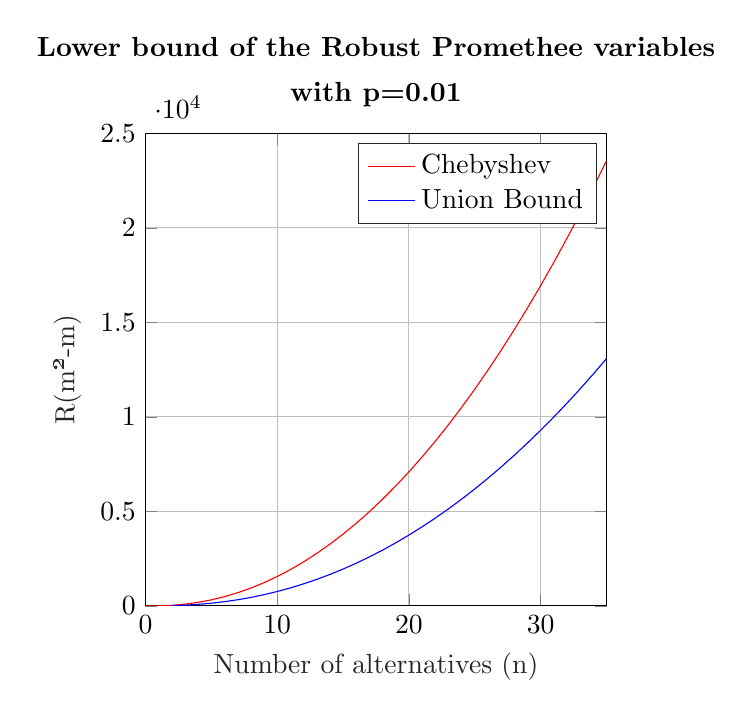
\begin{tikzpicture}

\begin{axis}[%
width=0.976\figurewidth,
height=\figureheight,
at={(0\figurewidth,0\figureheight)},
scale only axis,
unbounded coords=jump,
xmin=0,
xmax=35,
xlabel style={font=\color{white!15!black}},
xlabel={Number of alternatives (n)},
ymin=0,
ymax=25000,
ylabel style={font=\color{white!15!black}},
ylabel={R(m²-m)},
axis background/.style={fill=white},
title style={font=\bfseries, align=center},
title={Lower bound of the Robust Promethee variables\\[1ex]with p=0.01},
xmajorgrids,
ymajorgrids,
legend style={legend cell align=left, align=left, draw=white!15!black}
]
\addplot [color=red]
  table[row sep=crcr]{%
0	0\\
1	0\\
2	27.6509966032373\\
3	87.9529898097119\\
4	183.305979619424\\
5	315.089331111738\\
6	484.311818845429\\
7	691.775994268018\\
8	938.149483072761\\
9	1224.00413988576\\
10	1549.8401775453\\
11	1916.10215648992\\
12	2323.19014433359\\
13	2771.4678190237\\
14	3261.26854061302\\
15	3792.90001921513\\
16	4366.64798135329\\
17	4982.77910233012\\
18	5641.54338838129\\
19	6343.17613821827\\
20	7087.8995775081\\
21	7875.92423519082\\
22	8707.45011329402\\
23	9582.66768959483\\
24	10501.7587835311\\
25	11464.8973091509\\
26	12472.2499339324\\
27	13523.9766585368\\
28	14620.2313296609\\
29	15761.1620959022\\
30	16946.9118147781\\
31	18177.6184176372\\
32	19453.4152380778\\
33	20774.4313085827\\
34	22140.7916293437\\
35	23552.6174126463\\
};
\addlegendentry{Chebyshev}

\addplot [color=blue]
  table[row sep=crcr]{%
0	nan\\
1	nan\\
2	9.21034037197618\\
3	34.2226948479372\\
4	76.7631558625937\\
5	138.155105579643\\
6	219.396611612709\\
7	321.287090195884\\
8	444.492982985145\\
9	589.585616959982\\
10	757.064940818257\\
11	947.375370834262\\
12	1160.91689049792\\
13	1398.05312597772\\
14	1659.1174040359\\
15	1944.41741259058\\
16	2254.23886290483\\
17	2588.84841950897\\
18	2948.49608085844\\
19	3333.41713993184\\
20	3743.83381809646\\
21	4179.95664101634\\
22	4641.98560818757\\
23	5130.1111954061\\
24	5644.51522054129\\
25	6185.37159638658\\
26	6752.84698940659\\
27	7347.10139943668\\
28	7968.28867249541\\
29	8616.55695661894\\
30	9292.04910885679\\
31	9994.90306016517\\
32	10725.2521438113\\
33	11483.2253919972\\
34	12268.9478046751\\
35	13082.5405939251\\
};
\addlegendentry{Union Bound}

%test
\end{axis}
\end{tikzpicture}

    \caption{lower bound for R and m}
    \label{fig:bounds_on_Rm}
\end{figure}

It can be seen that for sets of 20 alternatives, $R(m^2-m)$ should be higher than about 3750.
This does not correspond to the values that have been found during the empirical investigation of the previous section where the optimal values of $R$ had to be more or less equal to $5000$ (which would lead $R(m^2-m)$ to be equal to $1e5$ when $m$ is equal to $5$).

This should not be surprising as the bound that have been found only guarantees that the probability that at least one couple of alternatives has not been evaluated during the procedure is under $1\%$, in other words, that the probability that all couples of alternatives have not been compared at least once is under $1\%$.
Of course, each couple of alternatives should be evaluated more than once in order for the matrix $P$ to correctly represent the probabilities of the alternatives to be ranked before others.

The bound found should therefore more be seen as a strict minimum for the methods usability, and certainly not as an optimal value.

\subsection{Non respect of the dominance relation}

As already shown, \textsc{promethee ii} respects the natural dominance relation (see section \ref{sec:pii_respect_dominance}).
Unfortunately, \textsc{robust promethee} on the other hand is not guaranteed to necessarily respect this relation.
The following paragraphs will give an example of an application where an alternative $a_w$, which dominates slightly another alternative $a_{w^{\prime}}$, will be ranked after this other alternative.

The evaluations of the alternatives considered for the example are given in Table \ref{tbl:monotonicity_counter_ex_ini}.


\begin{table}[h]
    \centering
    \begin{tabular}{@{\hskip 1cm} C @{\hskip 1cm}C C C C C@{\hskip 1cm}}
        \toprule
        a        & f_1(.)               & \dots  & f_c(.)        & \dots  & f_k(.) \\ [7pt]
        \midrule
        a_1      & f_1(a_1)             & \dots  & f_c(a_1)      & \dots  & f_k(a_1)\\
        \vdots   & \vdots               & \ddots & \vdots        & \ddots & \vdots \\
        a_{t_1}  & f_1(a_{t_1})         & \dots  & f_c(a_{t_1})  & \dots  & f_k(a_{t_1})  \\
        a_{t_2}  & f_1(a_{t_2})         & \dots  & f_c(a_{t_2})  & \dots  & f_k(a_{t_2})  \\
        \vdots   & \vdots               & \ddots & \vdots        & \ddots & \vdots \\
        a_{t_x}  & f_1(a_{t_x})         & \dots  & f_c(a_{t_x})  & \dots  & f_k(a_{t_x})  \\
        \vdots   & \vdots               & \ddots & \vdots        & \ddots & \vdots \\
        a_w      & f_1(a_w)             & \dots  & f_c(a_w)      & \dots  & f_k(a_w)  \\
        a_{w^{\prime}}    & f_1(a_w)             & \dots  & <f_c(a_w)      & \dots  & f_k(a_w)  \\
        \vdots   & \vdots               & \ddots & \vdots        & \ddots & \vdots \\
        a_n      & f_1(a_n)             & \dots  & f_c(a_n)      & \dots  & f_k(a_n)\\
        \bottomrule
    \end{tabular}
    \caption{Evaluation table of a set of alternatives not necessarily respecting the dominance relation with the \textsc{robust promethee} method}
    \label{tbl:monotonicity_counter_ex_ini}
\end{table}

This set $A$ of alternatives cannot be any set. It must include the following alternatives:

\begin{description}
    \item[$a_w$, $a_{w^{\prime}}$: ] these two alternatives are our witnesses as the dominated alternative ($a_{w^{\prime}}$) will be ranked before the dominant one ($a_w$). However, to justify the assumptions that will be done in the rest of the reasoning, these two alternatives must be considered to be very similar one to the other (their evaluations are equal on all the criteria excepts $f_c$ where $a_w$ is slightly better).
    \item[$a_t$:] at least two alternatives written as $a_{t_1} \dots a_{t_x}$ must suffer from the rank reversal phenomenon with the alternatives $a_w$ and $a_{w^{\prime}}$ when the \textsc{promethee ii} method is applied on sets of $m$ alternatives chosen from $A$ (containing of course the concerned alternative $a_t$ and $a_w$ or $a_{w^{\prime}}$).
\end{description}

The characterisation of the alternatives $a_t$ has the following consequence. During the application of the \textsc{robust promethee} procedure, at some iterations the alternatives $a_w$ and $a_{w^{\prime}}$ could be ranked before some alternative from $a_t$, and at some other iterations they could be ranked after some alternative from $a_t$.

Now suppose that at each of the $r=1 \dots R$ iterations one of the following cases happen:

\begin{enumerate}
    \item If both $a_w$ and $a_{w^{\prime}}$ are selected in the $m$ random alternatives, then no alternative $a_t$ is selected:
        \begin{equation}
            \big(A_{mr}(a_w) \cdot A_{mr}(a_{w^{\prime}})\big)\cdot \sum_{t=t_1}^{t_x}A_{mr}(a_t) = 0
        \end{equation}

    \item If $a_w$ and one alternative $a_t$ are selected in the $m$ random alternatives, then $a_w$ will be ranked after the alternative from $a_t$ at this iteration.

        \begin{equation}
            A_{mr}(a_w)\cdot A_{mr}(a_t) = 1
                \Rightarrow Beats_r(a_t, a_w) = 1 \qquad \forall t=t_1 \dots t_x
        \end{equation}

        This means that the alternatives $a_t$ will always be ranked before the alternative $a_w$ and that the following elements of the matrix $P$ will have the following values:  

        \begin{equation}
        p_{wt} = 0 \qquad p_{tw} = 1 \qquad  \forall t=t_1 \dots t_x
        \end{equation}

    \item If $a_{w^{\prime}}$ and one alternative $a_t$ are selected in the $m$ random alternatives, then $a_{w^{\prime}}$ will be ranked before the alternative from $a_t$ at this iteration.

        \begin{equation}
            A_{mr}(a_{w^{\prime}})\cdot A_{mr}(a_t) = 1
                \Rightarrow Beats_r(a_{w^{\prime}}, a_t) = 1 \qquad \forall t=t_1 \dots t_x
        \end{equation}

        This means that the alternatives $a_t$ will always be ranked after the alternative $a_{w^{\prime}}$ and that the following elements of the matrix $P$ will have the following values:  
        \begin{equation}
        p_{{w^{\prime}}t} = 1    \qquad  p_{t{w^{\prime}}} = 0   \qquad  \forall t=t_1 \dots t_x
        \end{equation}
\end{enumerate}

It will also be assumed, that since $a_w$ and $a_{w^{\prime}}$ are similar one to the other, they will obtain similar rankings when compared with the other alternatives:

\begin{equation}
        p_{{w^{\prime}}i} \simeq p_{wi} \qquad p_{i{w^{\prime}}} \simeq p_{iw}   \qquad   \forall i \neq w, {w^{\prime}}, t_1 \dots t_x
    \label{eqn:p_wt}
\end{equation}

Finally, it should also be noted that $p_{ww^\prime}$ is not always strictly equal to $1$ but will lie between $[0.5, 1]$ even if $a_{w^\prime}$ is dominated by $a_w$.
This is due to the fact that $Beats_r(a_w, a_{w^\prime})$ can be equal to $0.5$ since two alternatives dominating each other could obtain the same ranking (see equations (\ref{eqn:ai_dominates_aj}) and (\ref{eqn:beats_r})).

When computing the difference between the robust flows of $a_w$ and $a_{w^{\prime}}$ computed on the probability matrix, the following results will be obtained:

\begin{equation}
    \begin{split}
        \phi_{rob}(a_{w^{\prime}}) - \phi_{rob}(a_w) & =
            \frac{1}{n-1} \sum\limits_{i=1}^n \left[ (p_{{w^{\prime}}i} - p_{i{w^{\prime}}}) -(p_{wi} - p_{iw}) \right] \\
        & \simeq \frac{1}{n-1} \sum\limits_{t=t_1}^{t_x} \left[(p_{{w^{\prime}}t} - p_{t{w^{\prime}}})
            - (p_{{w^{\prime}}t} - p_{t{w^{\prime}}}) \right] \\
        & \qquad + \frac{1}{n-1}\big((p_{ww^\prime} - p_{w^\prime w}) -  (p_{w^\prime w} - p_{ww^\prime})\big) \\
        & \ge \frac{1}{n-1}\big[\sum\limits_{t=t_1}^{t_x} 2 - 2\big] \\
        & > 0
    \end{split}
    \label{eqn:non_dominance}
\end{equation}

The last inequality is justified by the hypothesis of this example which stated that the set $a_t = a_{t_{1}} \dots a_{t_{x}}$ was composed of at least two alternatives.

It can therefore be seen from this example that the dominance relation could be violated by the \textsc{robust promethee} method.
This phenomenon is closely related to the presence of rank reversal in \textsc{promethee ii}. 
In fact, it is also related to some form of nontransivity.
The dominated alternative $a_{w^\prime}$ cannot be ranked before the dominant alternative $a_w$ in one of the subsets, but it can be ranked before some alternatives $a_t$. These alternatives $a_t$, on the other hand, can be ranked before $a_w$ in some subsets.

However, even when there exists alternatives $a_t$ which can be ranked before or after some alternatives $a_w$ and $a_{w^\prime}$ depending on the subsets, $a_w$ will always have a probability at least as great of being ranked before $a_t$ than $a_{w^\prime}$.
Therefore, since the \textsc{robust promethee} method must be employed with $R$ relatively high, unbalanced repartition of the samples that could lead to violations of the dominance relation are not likely to happen in practical problems.

\section{Synthesis of the \textsc{robust promethee} method and conclusion}

After having studied \textsc{robust promethee} mathematically and using empirical results, we can conclude that it has some advantages and some drawbacks which both should be mitigated.

First, it can be said that this method seems, up to a certain point, to be succeeding in its purpose of reducing the number of rank reversals.
The improvement is however not always as drastic as first observed with the \textsc{hdi} data set and it is neither guaranteed that the method will be effective on all data sets.

It has also been shown that the dominance relation was not necessarily respected and some counterintuitive rankings could be obtained. Such violations should however have very low probabilities to occur and have not yet been observed.

The most limiting characteristic of \textsc{robust promethee} that has been found is probably that the determination of appropriate parameters is not an easy task and vary from one data set to another.
Furthermore the variations of the best values of the parameter $m$ are not small variations. It has been seen that this optimal value could be equal to about $30\%$ of the size of the alternative set as it could also be equal to $80\%$.
This could be a serious obstacle for solving practical decision aid problems as the parameters that should be used will not be known in advance.

Finally, it should also be pointed out that the fact that some rank reversal are still occurring should not automatically discredit this method.
This chapter has mainly consisted in studying the quantity of rank reversal occurrences but it has also been seen that \textsc{robust promethee} was producing rankings relatively similar as \textsc{promethee ii}.
It should therefore still be studied if the rankings produced are satisfying or not (are they more satisfying than the ones produced by the original \textsc{promethee ii} method ?).

In the following chapter, a new method, \textsc{referenced promethee}, will be studied.
This method handles the rank reversal problem with a different approach.
Instead of building a ranking similar to the one produced by \textsc{promethee ii} and trying to reduce the number of rank reversal, by construction, \textsc{referenced promethee} avoids any rank reversal. 
It will however be studied if it can produce rankings similar to the ones produced by \textsc{promethee ii}.






